\documentclass[11pt,a4paper]{report}

\usepackage[margin=1in]{geometry}
\usepackage[T1]{fontenc}
\usepackage[utf8]{inputenc}
\usepackage{lmodern}
\usepackage{microtype}
\usepackage{amsmath,amssymb,mathtools}
\usepackage{graphicx}
\usepackage[table]{xcolor}
\usepackage{booktabs,longtable,array,tabularx}
\usepackage{enumitem}
\usepackage{float}
\usepackage{subcaption}
\usepackage{siunitx}
\usepackage{tikz}
\usepackage{pgfplots}
\usepackage{hyperref}
\usepackage[nameinlink,noabbrev]{cleveref}

\pgfplotsset{compat=1.18}
\sisetup{round-mode=places,round-precision=4}
\hypersetup{
  colorlinks=true,
  linkcolor=black,
  citecolor=black,
  urlcolor=black,
  pdftitle={BERT-Based Hotel Review Classification},
  pdfauthor={Arka Braja Prasad Nath and Farhan Tahmid},
  pdfsubject={CSE 4122 Natural Language Processing Laboratory project report}
}

% Required diagram palette.
\definecolor{PaletteGray}{HTML}{E0E0E0}
\definecolor{PaletteCyan}{HTML}{97ECF8}
\definecolor{PaletteOrange}{HTML}{FFD0AC}
\definecolor{PaletteRed}{HTML}{FFA0A0}
\definecolor{PaletteYellow}{HTML}{FFF17B}
\definecolor{PalettePurple}{HTML}{ACA7FF}
\definecolor{PaletteGreen}{HTML}{A4FFA1}
\definecolor{PalettePink}{HTML}{F4C5FF}

\newcommand{\R}{\mathbb{R}}
\newcommand{\code}[1]{\texttt{#1}}
\newcommand{\sourcepath}[1]{\path{#1}}
\newcommand{\aspectcm}[5]{%
  \begin{minipage}[t]{0.31\textwidth}
  \centering\small
  \textbf{#1}\par\vspace{2pt}
  \renewcommand{\arraystretch}{1.12}
  \begin{tabular}{c|rr}
    & \multicolumn{2}{c}{Predicted} \\
    & No & Yes \\
    \hline
    True no  & \cellcolor{PaletteGreen}#2 & \cellcolor{PaletteRed}#3 \\
    True yes & \cellcolor{PaletteYellow}#4 & \cellcolor{PaletteGreen}#5
  \end{tabular}
  \end{minipage}%
}

\begin{document}

\hypersetup{pageanchor=false}
\begin{titlepage}
\centering

\includegraphics[width=0.18\textwidth]{kuet_logo.png}\par
\vspace{0.45cm}
{\Large\bfseries Khulna University of Engineering \& Technology\par}
\vspace{0.18cm}
{\large\bfseries Department of Computer Science and Engineering\par}
\vspace{0.85cm}
{\LARGE\bfseries PROJECT REPORT\par}
\vspace{0.65cm}
{\large\bfseries Title:\par}
\vspace{0.15cm}
{\LARGE\bfseries BERT-Based Hotel Review Classification\par}
\vspace{0.8cm}

\renewcommand{\arraystretch}{1.35}
\begin{tabular}{@{}ll@{}}
\textbf{Course No:} & CSE 4122 \\
\textbf{Course Title:} & Natural Language Processing Laboratory \\
\textbf{Submission Date:} & 23 Sept, 2026 \\
\end{tabular}

\vfill
\begin{minipage}[t]{0.48\textwidth}
\raggedright
\textbf{Submitted To:}\par
\vspace{0.2cm}
\textbf{Dr. K. M. Azharul Hasan}\par
Professor, Dept. of CSE, KUET\par
\vspace{0.45cm}
\textbf{Md Nazirulhasan Shawon}\par
Assistant Professor, Dept. of CSE, KUET
\end{minipage}
\hfill
\begin{minipage}[t]{0.43\textwidth}
\raggedright
\textbf{Submitted By:}\par
\vspace{0.2cm}
Arka Braja Prasad Nath (2107055)\par
Farhan Tahmid (2107059)
\end{minipage}
\vspace{0.55cm}
\end{titlepage}

\begin{abstract}
This project solves two related natural-language classification tasks over hotel-review sentences.  A sentiment model selects exactly one class from \emph{negative}, \emph{neutral}, and \emph{positive}; a separate aspect model independently detects any subset of 21 hotel aspects.  Both models fine-tune \code{bert-base-uncased} with a maximum input length of 128 tokens.  The sentiment branch uses a three-way softmax and cross-entropy, whereas the aspect branch uses 21 sigmoids and binary cross-entropy with logits.  The cleaned HRAST corpus contains 23,095 unique, valid reviews and is split into 16,227 training, 3,441 validation, and 3,427 test records by iterative multilabel stratification.  The executed notebook reports sentiment accuracy of 0.9387 and macro-F1 of 0.7258, and aspect macro-F1 of 0.8825 and micro-F1 of 0.8941 at threshold 0.30.  It also exports both classifiers in the Hugging Face format required by the inference application and verifies that a reloaded model reproduces the in-memory output.
\end{abstract}

\hypersetup{pageanchor=true}
\pagenumbering{roman}
\tableofcontents
\listoffigures
\listoftables
\clearpage
\pagenumbering{arabic}

\chapter{Introduction}

Hotel reviews often express an overall opinion while mentioning several concrete service attributes.  These are different prediction structures:
\begin{align}
  \text{sentiment} &: x \longmapsto y^{(s)} \in \{0,1,2\},\\
  \text{aspects} &: x \longmapsto \mathbf{y}^{(a)} \in \{0,1\}^{21}.
\end{align}
The first is single-label multiclass classification.  The second is multilabel classification: several entries in \(\mathbf{y}^{(a)}\) may be one, or every entry may be zero.  For example, ``Breakfast was poor but the staff were excellent'' may activate both \emph{Breakfast} and \emph{Staff}, even though only one dominant sentiment is returned.

The primary implementation examined in this report is the executed notebook \sourcepath{notebooks/farhan-koice-hoice.ipynb}.  The interactive inference application is \sourcepath{inference_app/app.py}; the repository also contains a Flask path through \sourcepath{src/web/app.py} and \sourcepath{src/inference/predictor.py}.  The mathematical description, procedural details, plots, and measured final metrics below follow this updated notebook.  The complete project source is available in the \href{https://github.com/MishtiAloo/Hotel-Review-Classification.git}{GitHub repository}.

\section{Project outputs}

The executed training stage produces two Hugging Face checkpoint directories under \sourcepath{/kaggle/working/artifacts}:
\begin{itemize}[leftmargin=*]
  \item \sourcepath{artifacts/sentiment}: tokenizer, configuration, and a BERT model with three output logits;
  \item \sourcepath{artifacts/aspects}: tokenizer, configuration, a BERT model with 21 output logits, and threshold metadata.
\end{itemize}
The Streamlit demo loads both models once, runs both over each submitted review, and visualizes the resulting probabilities.

\chapter{Dataset and Preparation}

The HRAST data file is distributed through the \href{https://www.kaggle.com/datasets/costastziouvas/hotel-reviews-aspects-sentiments-and-topics?select=HRAST.csv}{Hotel Reviews: Aspects, Sentiments and Topics dataset on Kaggle}.  The notebook recursively locates the attached \code{HRAST.csv} under \sourcepath{/kaggle/input/}; the recorded run found \sourcepath{/kaggle/input/datasets/arkaariya/hotel-review/HRAST.csv}, while the repository keeps its local copy at \sourcepath{dataset/HRAST.csv}.

\section{Label space}

The sentiment identifier order is
\[
0=\text{negative},\qquad 1=\text{neutral},\qquad 2=\text{positive}.
\]
The 21 aspect labels are Clean, Comfort, Facilities/Amenities, Location, Restaurant (dinner), Staff, View (Balcony), Breakfast, Room, Pool, Beach, Bathroom/Shower (toilet), Bar, Bed, Parking, Noise, Reception-checkin, Lift, Value for money, Wi-Fi, and Generic.  This order is part of the checkpoint interface: output coordinate \(j\) must always be decoded with the same label used during training.

\section{Cleaning and quality controls}

The notebook performs the following necessary preparation before any split is made:
\begin{enumerate}[leftmargin=*]
  \item Read \code{HRAST.csv} with \code{utf-8-sig} and remove unnamed export columns.
  \item Convert review values to strings, trim the ends, collapse every run of whitespace to one space, and discard empty reviews.
  \item Require every one of the 24 target cells (three sentiment and 21 aspect fields) to be binary.
  \item Require the three sentiment flags to sum to exactly one, then map the one-hot values to a class name.
  \item Group rows by exact cleaned review text.  Keep one copy if every duplicate annotation agrees; discard the entire group if any copy conflicts.
\end{enumerate}

The executed cleaning cells show 23,113 raw and non-empty rows, 23,112 rows after the binary-label check, 23,108 rows after enforcing exactly one sentiment label, and 23,095 rows after duplicate resolution.  Thus 18 rows are removed in total.  The staged checks are important because a row can pass the binary constraint but still have zero or several active sentiment flags.
Deduplication is completed before splitting, which prevents identical reviews from leaking between train and evaluation sets.

\section{Stratified split}

The splitter receives a 24-dimensional target matrix containing all aspect and sentiment indicators.  Iterative multilabel stratification is used because ordinary single-class stratification cannot jointly preserve 21 overlapping aspect frequencies \cite{sechidis2011}.

\begin{table}[H]
\centering
\caption{Split sizes produced by the updated notebook.}
\label{tab:splits}
\begin{tabular}{lrrr}
\toprule
Split & Rows & Fraction & Intended use \\
\midrule
Training & 16,227 & 70.26\% & Parameter estimation \\
Validation & 3,441 & 14.90\% & Checkpoint and threshold selection \\
Test & 3,427 & 14.84\% & Final, one-time evaluation \\
\midrule
Total & 23,095 & 100.00\% & \\
\bottomrule
\end{tabular}
\end{table}

The rare neutral class is a central difficulty.  Across the cleaned corpus, the counts are 11,808 positive, 10,496 negative, and only 791 neutral reviews.  This imbalance explains why accuracy alone is insufficient and why macro-F1 is used for model selection.

\begin{figure}[H]
\centering
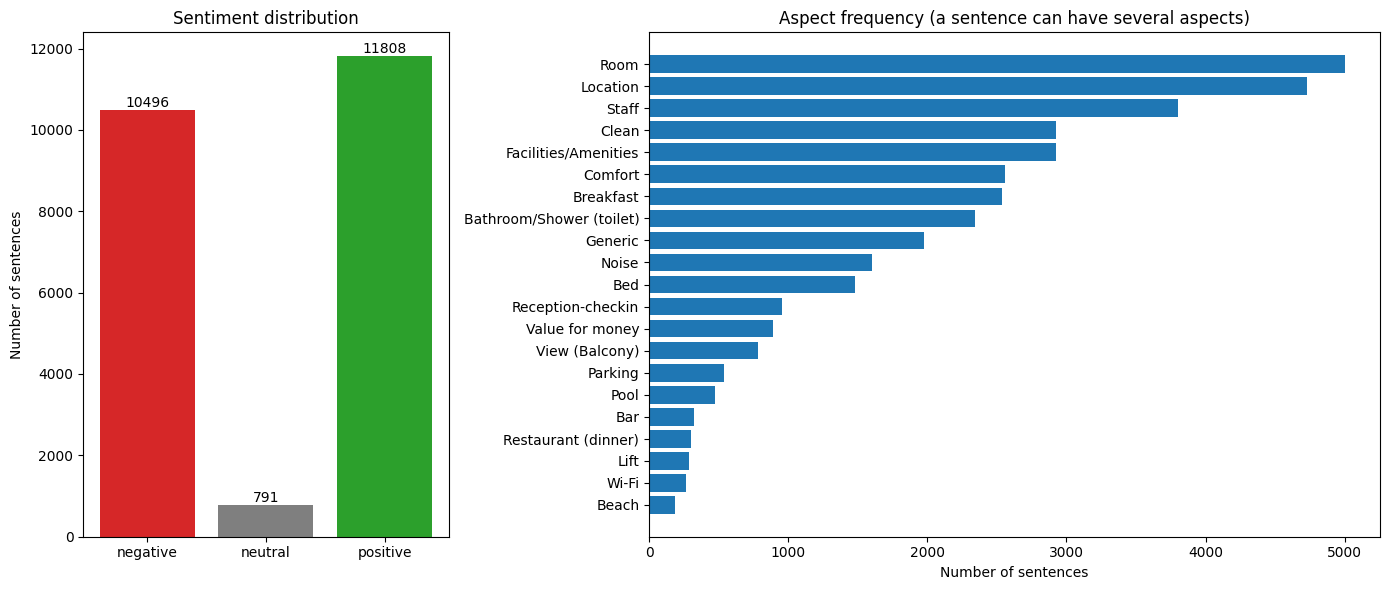
\includegraphics[width=\textwidth]{notebook_data_distribution.png}
\caption{Sentiment and aspect distributions computed over the 23,095 cleaned reviews by the updated notebook.  The large variation motivates multilabel stratification and macro-averaged evaluation.}
\label{fig:data-distribution}
\end{figure}

\begin{figure}[H]
\centering
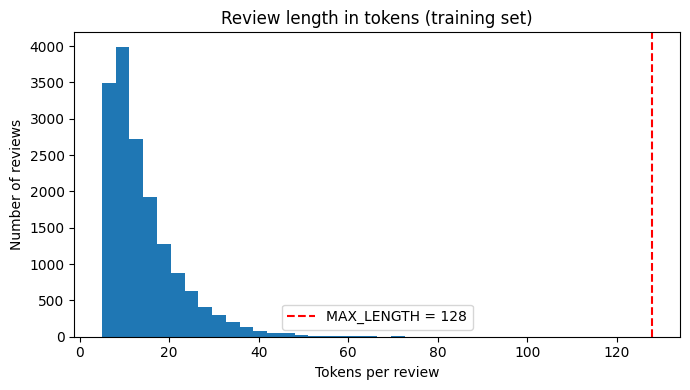
\includegraphics[width=0.82\textwidth]{notebook_review_lengths.png}
\caption{Training-set WordPiece lengths after truncation.  The mean is 14.5 tokens, the maximum is 128, and only one of 16,227 training reviews reaches the configured limit.}
\label{fig:review-lengths}
\end{figure}

\chapter{Model Architecture}

\section{Input representation}

For a batch size \(B\) and a dynamically padded sequence length \(L\leq128\), tokenization produces
\[
  \mathbf{I},\mathbf{M}\in\mathbb{N}^{B\times L},
\]
where \(\mathbf{I}\) contains WordPiece identifiers and \(\mathbf{M}\) is the attention mask.  The BERT embedding at position \(i\) is the sum
\begin{equation}
  \mathbf{x}_i=\mathbf{e}^{\mathrm{token}}_i+
  \mathbf{e}^{\mathrm{position}}_i+
  \mathbf{e}^{\mathrm{segment}}_i \in \R^{768}.
\end{equation}
The first token is \code{[CLS]} and the last content boundary is \code{[SEP]}.  The notebook tokenizes every split once and caches variable-length ID lists.  Its hand-written \code{pad\_batch} function then pads only to the longest item in the current batch and constructs \(\mathbf{M}\) by comparing every ID with the tokenizer's padding ID; masked positions do not contribute to attention.

\section{BERT-base encoder}

The project uses the pretrained uncased BERT-base encoder \cite{devlin2019}: 12 Transformer blocks, hidden width \(d=768\), 12 attention heads, head width \(d_h=64\), and feed-forward width 3,072.  For one head in one block,
\begin{align}
  \mathbf{Q}&=\mathbf{X}\mathbf{W}^{Q}, &
  \mathbf{K}&=\mathbf{X}\mathbf{W}^{K}, &
  \mathbf{V}&=\mathbf{X}\mathbf{W}^{V},\\
  \operatorname{Attention}(\mathbf{Q},\mathbf{K},\mathbf{V})
  &=\operatorname{softmax}\!\left(\frac{\mathbf{Q}\mathbf{K}^{\top}}{\sqrt{d_h}}+\mathbf{A}\right)\mathbf{V},
\end{align}
where \(\mathbf{A}\) applies a large negative value to masked key positions.  The 12 heads are concatenated and projected:
\begin{equation}
  \operatorname{MHA}(\mathbf{X})=
  \operatorname{Concat}(\mathrm{head}_1,\ldots,\mathrm{head}_{12})\mathbf{W}^{O}.
\end{equation}
After a residual connection and layer normalization, the position-wise network is
\begin{equation}
  \operatorname{FFN}(\mathbf{h})=
  \operatorname{GELU}(\mathbf{h}\mathbf{W}_1+\mathbf{b}_1)\mathbf{W}_2+\mathbf{b}_2,
\end{equation}
with dimensions \(768\rightarrow3072\rightarrow768\), followed by another residual connection and layer normalization.

\begin{figure}[H]
\centering
\makebox[\textwidth][c]{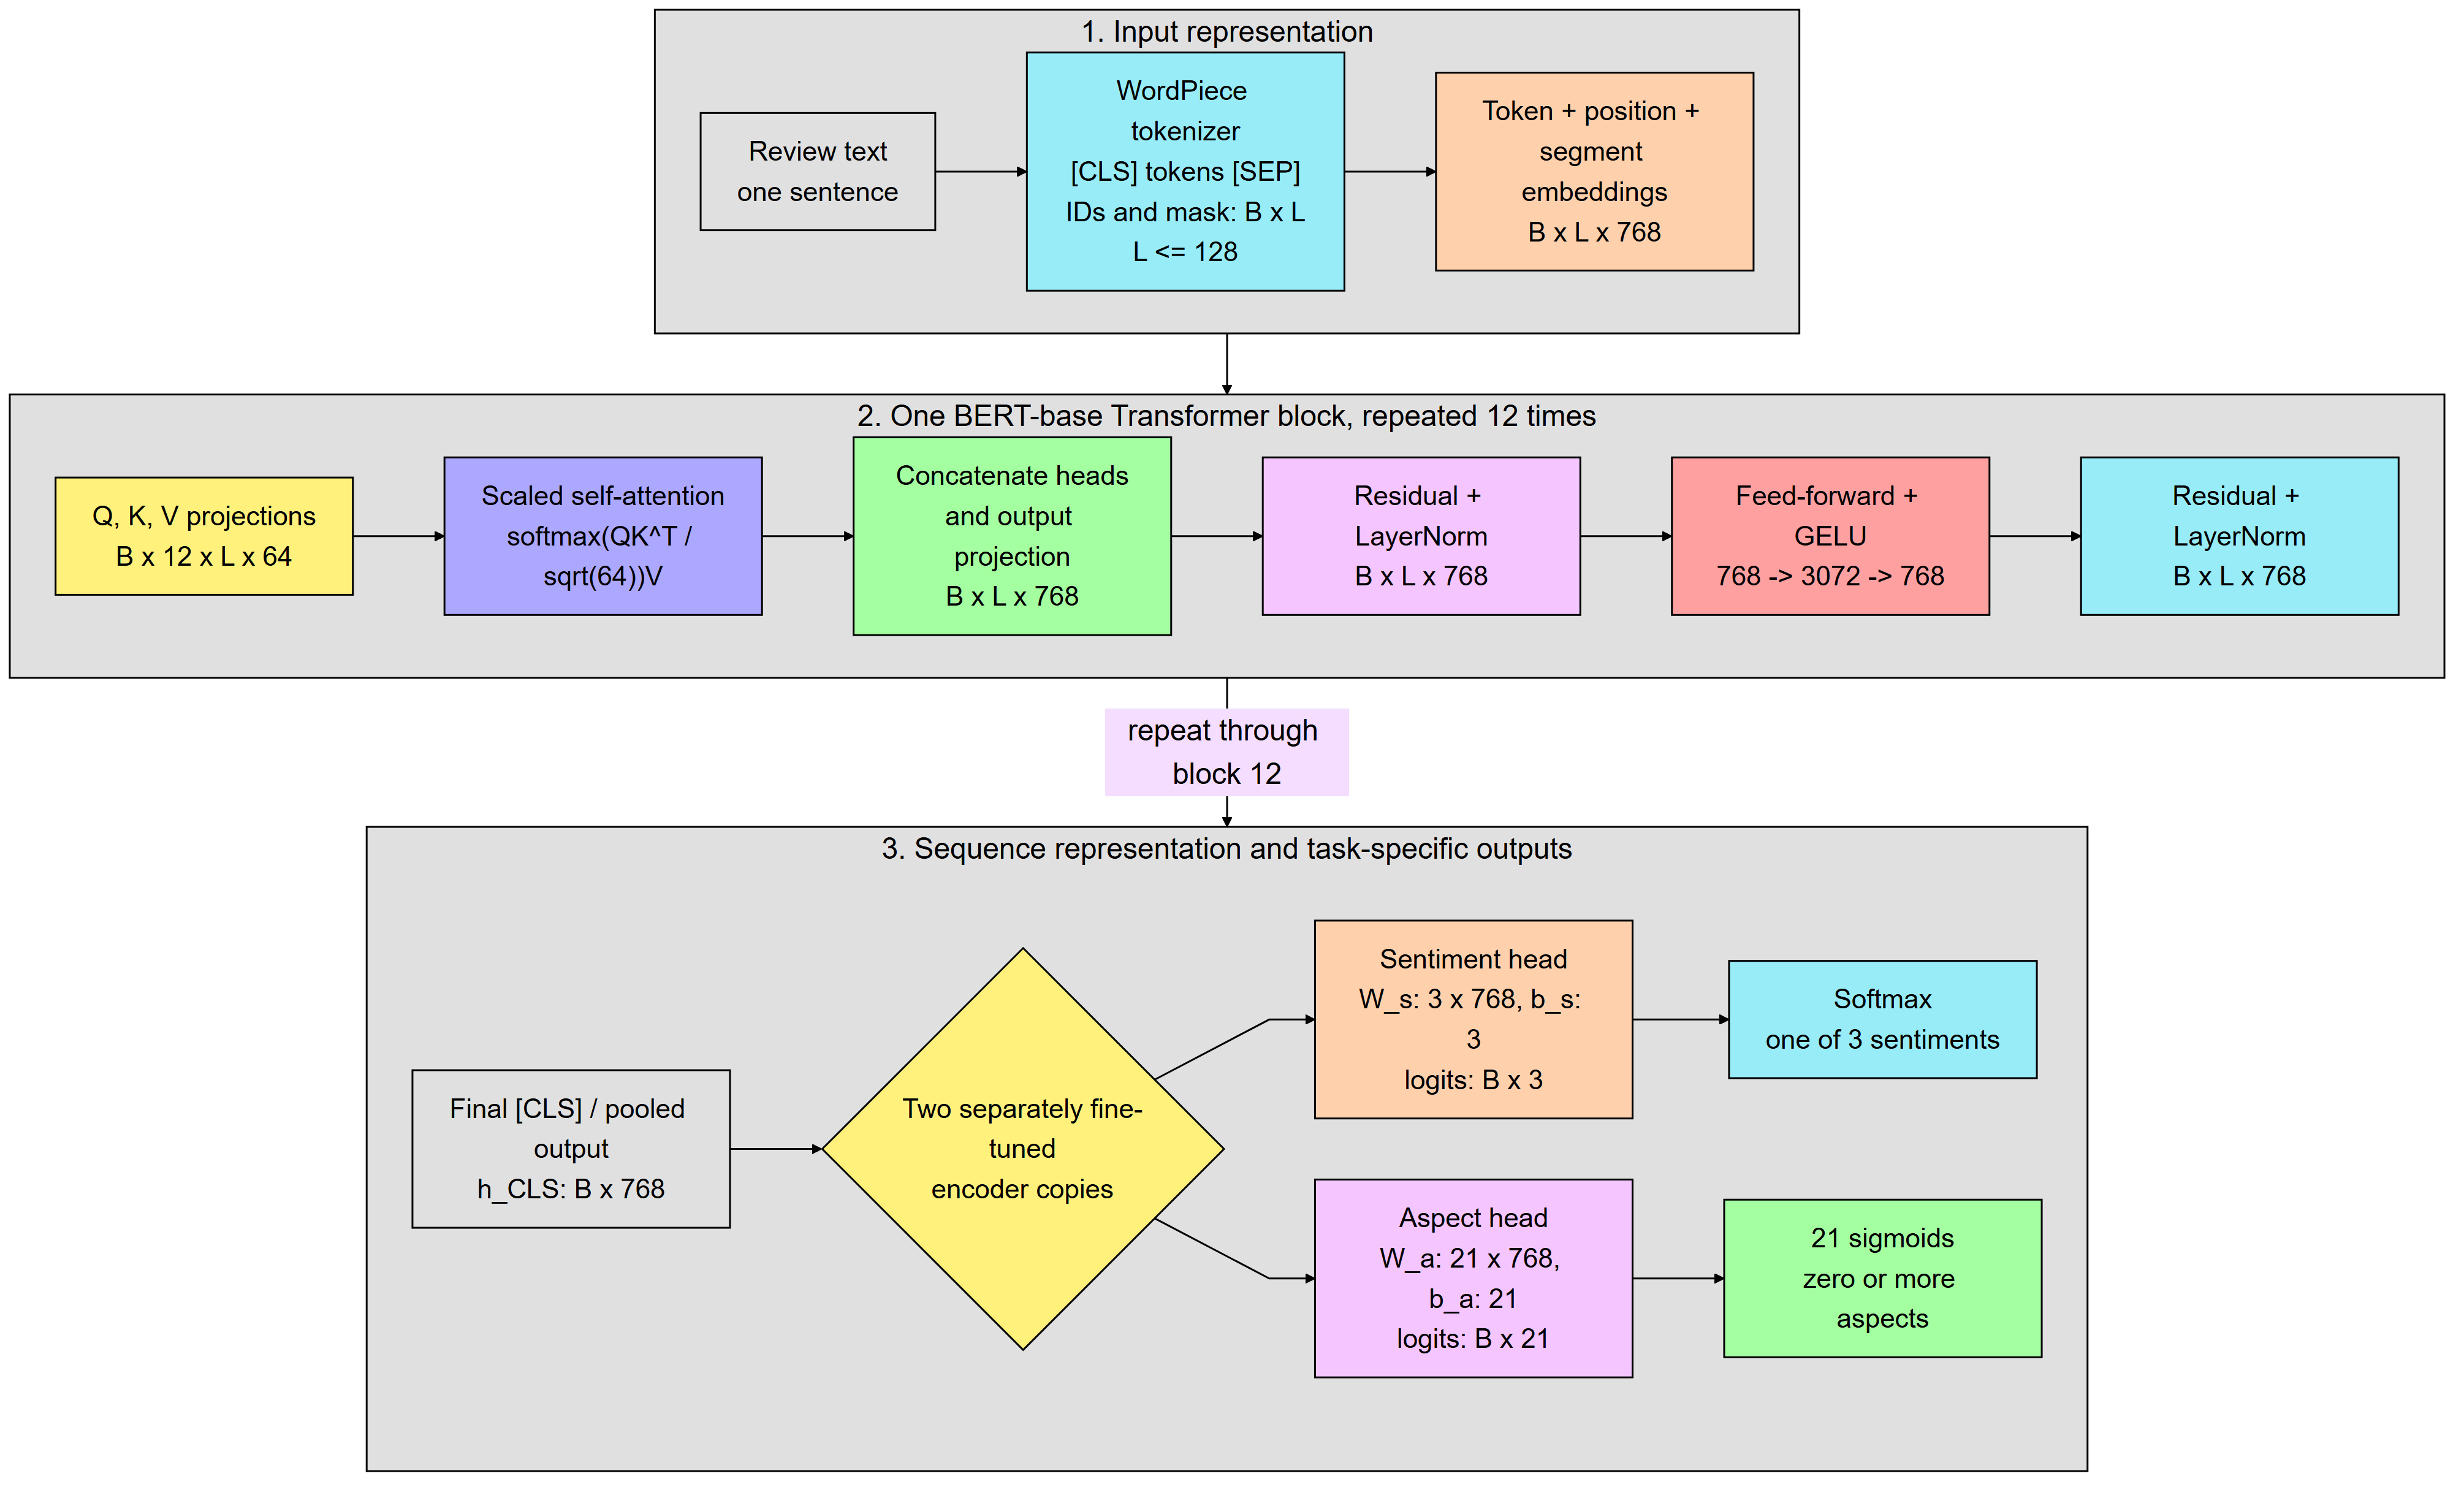
\includegraphics[width=1.18\textwidth,height=0.82\textheight,keepaspectratio]{bert_architecture.png}}
\caption[Simplified BERT and classification architecture.]{Simplified BERT and classification architecture with batch-dependent tensor dimensions.  The sentiment and aspect systems are separately fine-tuned copies, not two heads sharing one encoder at runtime.  Mermaid source: \code{bert\_architecture.mmd}.}
\label{fig:bert-architecture}
\end{figure}

\section{Classification heads}

Let \(\mathbf{h}_{\mathrm{CLS}}\in\R^{B\times768}\) denote the final pooled representation.  With dropout \(D(\cdot)\), the sentiment logits are
\begin{equation}
  \mathbf{z}^{(s)}=D(\mathbf{h}_{\mathrm{CLS}})\mathbf{W}_s^{\top}+\mathbf{b}_s,
  \quad \mathbf{W}_s\in\R^{3\times768},\quad \mathbf{z}^{(s)}\in\R^{B\times3}.
\end{equation}
The aspect head has the analogous form
\begin{equation}
  \mathbf{z}^{(a)}=D(\mathbf{h}_{\mathrm{CLS}})\mathbf{W}_a^{\top}+\mathbf{b}_a,
  \quad \mathbf{W}_a\in\R^{21\times768},\quad \mathbf{z}^{(a)}\in\R^{B\times21}.
\end{equation}
The hand-written \code{BertClassifier} obtains \(\mathbf{h}_{\mathrm{CLS}}\) from \code{BertModel.pooler\_output}, applies dropout with probability 0.1, and then applies the appropriate linear head.  Head weights are initialized from \(\mathcal{N}(0,0.02^2)\) and biases from zero, while the encoder begins with pretrained weights.  Each task owns its complete BERT encoder and head, so training and deployment store roughly 110 million parameters per model.

\chapter{Objectives and Optimization}

\section{Sentiment softmax and cross-entropy}

For review \(i\), softmax converts the three logits into a categorical distribution:
\begin{equation}
  p^{(s)}_{ic}=\frac{\exp(z^{(s)}_{ic})}
  {\sum_{k=1}^{3}\exp(z^{(s)}_{ik})},\qquad c\in\{1,2,3\}.
\end{equation}
The probabilities sum to one.  Inference returns
\begin{equation}
  \widehat{y}^{(s)}_i=\arg\max_c p^{(s)}_{ic}.
\end{equation}
For one-hot target \(y^{(s)}_{ic}\), the mean multiclass cross-entropy is
\begin{equation}
  \mathcal{L}_{\mathrm{CE}}=-\frac{1}{B}\sum_{i=1}^{B}
  \sum_{c=1}^{3}y^{(s)}_{ic}\log p^{(s)}_{ic}
  =-\frac{1}{B}\sum_{i=1}^{B}\log p^{(s)}_{i,y_i}.
\end{equation}

\section{Aspect sigmoid and binary cross-entropy}

An aspect is not in competition with the other aspects.  Each logit is therefore transformed independently:
\begin{equation}
  p^{(a)}_{ij}=\sigma(z^{(a)}_{ij})=
  \frac{1}{1+\exp(-z^{(a)}_{ij})},\qquad j=1,\ldots,21.
\end{equation}
The notebook's \code{BCEWithLogitsLoss} combines the sigmoid and binary cross-entropy in a numerically stable operation:
\begin{equation}
  \mathcal{L}_{\mathrm{BCE}}=-\frac{1}{21B}
  \sum_{i=1}^{B}\sum_{j=1}^{21}
  \left[y^{(a)}_{ij}\log\sigma(z^{(a)}_{ij})+
  (1-y^{(a)}_{ij})\log(1-\sigma(z^{(a)}_{ij}))\right].
\end{equation}
With a selected threshold \(\tau_j\), the decision rule is
\begin{equation}
  \widehat{y}^{(a)}_{ij}=\mathbb{1}\!\left[p^{(a)}_{ij}\geq\tau_j\right].
\end{equation}
The updated notebook searches one global \(\tau\), then writes both \code{global\_threshold} and a 21-entry \code{per\_label\_thresholds} mapping to \sourcepath{aspects/thresholds.json}.  Every per-label value is initialized to the selected global threshold so both web interfaces can consume the same export.

\begin{figure}[H]
\centering
\begin{subfigure}{0.48\textwidth}
\centering
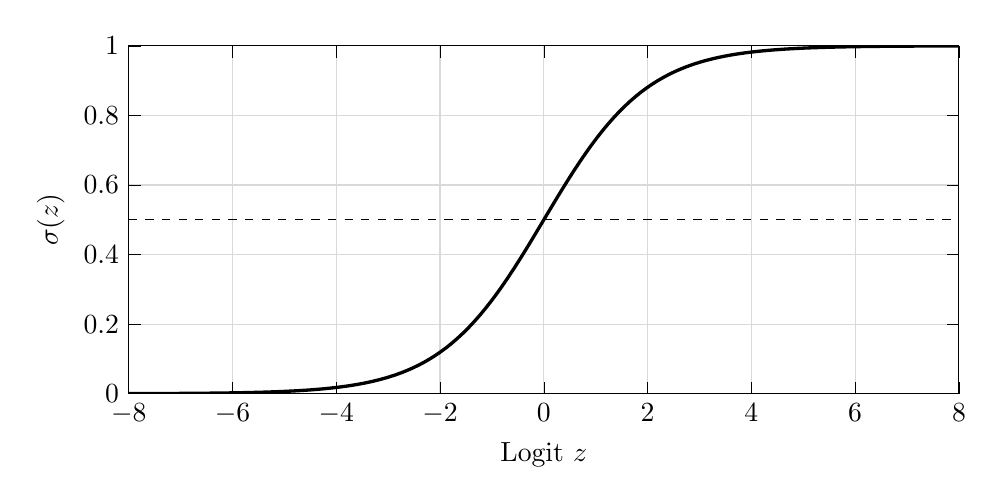
\begin{tikzpicture}
\begin{axis}[
 width=\textwidth,height=6cm,
 xlabel={Logit $z$},ylabel={$\sigma(z)$},
 xmin=-8,xmax=8,ymin=0,ymax=1,
 axis line style={black},tick style={black},grid=major,grid style={black!15}]
\addplot[domain=-8:8,samples=150,very thick,color=PalettePurple,draw=black] {1/(1+exp(-x))};
\addplot[dashed,black] coordinates {(-8,0.5) (8,0.5)};
\end{axis}
\end{tikzpicture}
\caption{Sigmoid probability.}
\end{subfigure}
\hfill
\begin{subfigure}{0.48\textwidth}
\centering
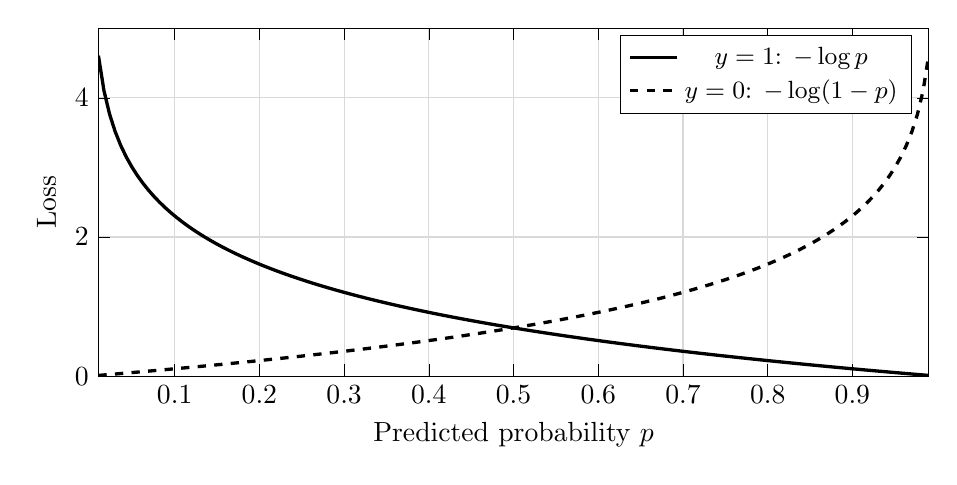
\begin{tikzpicture}
\begin{axis}[
 width=\textwidth,height=6cm,
 xlabel={Predicted probability $p$},ylabel={Loss},
 xmin=0.01,xmax=0.99,ymin=0,ymax=5,
 legend style={draw=black,fill=white,font=\small},
 axis line style={black},tick style={black},grid=major,grid style={black!15}]
\addplot[domain=0.01:0.99,samples=150,very thick,color=PaletteRed,draw=black] {-ln(x)};
\addlegendentry{$y=1$: $-\log p$}
\addplot[domain=0.01:0.99,samples=150,very thick,color=PaletteCyan,draw=black,dashed] {-ln(1-x)};
\addlegendentry{$y=0$: $-\log(1-p)$}
\end{axis}
\end{tikzpicture}
\caption{Binary cross-entropy terms.}
\end{subfigure}
\caption{Activation and loss-response curves.  These are analytic curves, not reconstructed training histories.}
\label{fig:analytic-curves}
\end{figure}

\section{Backpropagation and AdamW}

All BERT and classifier parameters are fine-tuned.  For parameter vector \(\boldsymbol\theta\) and minibatch loss \(\mathcal{L}_t\), backpropagation gives
\begin{equation}
  \mathbf{g}_t=\nabla_{\boldsymbol\theta}\mathcal{L}_t(\boldsymbol\theta_{t-1}).
\end{equation}
AdamW maintains exponential first and second moments \cite{loshchilov2019}:
\begin{align}
  \mathbf{m}_t&=\beta_1\mathbf{m}_{t-1}+(1-\beta_1)\mathbf{g}_t,\\
  \mathbf{v}_t&=\beta_2\mathbf{v}_{t-1}+(1-\beta_2)\mathbf{g}_t\odot\mathbf{g}_t,\\
  \widehat{\mathbf{m}}_t&=\frac{\mathbf{m}_t}{1-\beta_1^t},\qquad
  \widehat{\mathbf{v}}_t=\frac{\mathbf{v}_t}{1-\beta_2^t}.
\end{align}
Its decoupled weight-decay update can be written as
\begin{equation}
  \boldsymbol\theta_t=\boldsymbol\theta_{t-1}
  -\eta\frac{\widehat{\mathbf{m}}_t}{\sqrt{\widehat{\mathbf{v}}_t}+\epsilon}
  -\eta\lambda\boldsymbol\theta_{t-1}.
\end{equation}
The notebook specifies \(\eta=2\times10^{-5}\) and otherwise uses PyTorch AdamW defaults: \(\beta_1=0.9\), \(\beta_2=0.999\), \(\epsilon=10^{-8}\), and \(\lambda=0.01\).  The update is preceded by \code{zero\_grad()} and followed by the next forward pass.

\chapter{Training and Model Selection}

\section{Hyperparameters used by the updated notebook}

\begin{table}[H]
\centering
\caption{Training configuration in \code{notebooks/farhan-koice-hoice.ipynb}.}
\label{tab:hyperparameters}
\begin{tabular}{ll}
\toprule
Setting & Value \\
\midrule
Base encoder & \code{bert-base-uncased} \\
Maximum sequence length & 128 WordPiece tokens \\
Epochs & 5 \\
Learning rate & \(2\times10^{-5}\) \\
Training / evaluation batch size & 16 / 32 \\
Classifier dropout & 0.10 \\
Optimizer & AdamW \\
Sentiment objective & Cross-entropy \\
Aspect objective & BCE with logits \\
Checkpoint criterion & Validation macro-F1 \\
Seed & 42 \\
\bottomrule
\end{tabular}
\end{table}

The executed run used an NVIDIA Tesla T4.  The standalone \sourcepath{configs/train.yaml} contains additional settings such as batch size 32, warmup, gradient clipping, mixed precision, and early stopping.  Those settings do \emph{not} control the updated notebook; it uses only the constants in \cref{tab:hyperparameters}.  It runs all five epochs without a scheduler, gradient clipping, mixed precision, class weighting, or early stopping.

\section{End-to-end procedure}

Before training, the notebook tokenizes all reviews once with truncation at 128 tokens and no padding.  At the start of every epoch the hand-written batcher shuffles indices.  Each batch is dynamically padded, given an attention mask, moved to the selected CUDA or CPU device, passed through its task-specific model, differentiated, and updated.  Evaluation runs under \code{no\_grad()} with the model in evaluation mode.  Accuracy, precision, recall, F1, and confusion counts are computed by notebook functions rather than a metrics library.  The best checkpoint is replaced only when validation macro-F1 strictly improves.

For the aspect model, epoch selection first uses threshold 0.50.  After loading the best checkpoint, the notebook searches
\begin{equation}
  \mathcal{T}=\{0.20,0.25,\ldots,0.80\},\qquad
  \tau^*=\arg\max_{\tau\in\mathcal{T}}F_{1,\mathrm{macro}}^{\mathrm{val}}(\tau).
\end{equation}
The validation set is appropriate for this choice; the test set remains untouched until both checkpoint and threshold are fixed.  Whenever validation macro-F1 improves, \code{save\_for\_web} copies the trained encoder and head into a standard \code{AutoModelForSequenceClassification}, attaches semantic \code{id2label}, \code{label2id}, and \code{problem\_type} metadata, and saves the tokenizer.  The final aspect search selects \(\tau^*=0.30\); after held-out evaluation, the notebook writes metrics and threshold metadata, runs a standard-model reload smoke test, and packages both model folders as \code{hotel\_models.zip}.

\clearpage
\begin{figure}[H]
\centering
\makebox[\textwidth][c]{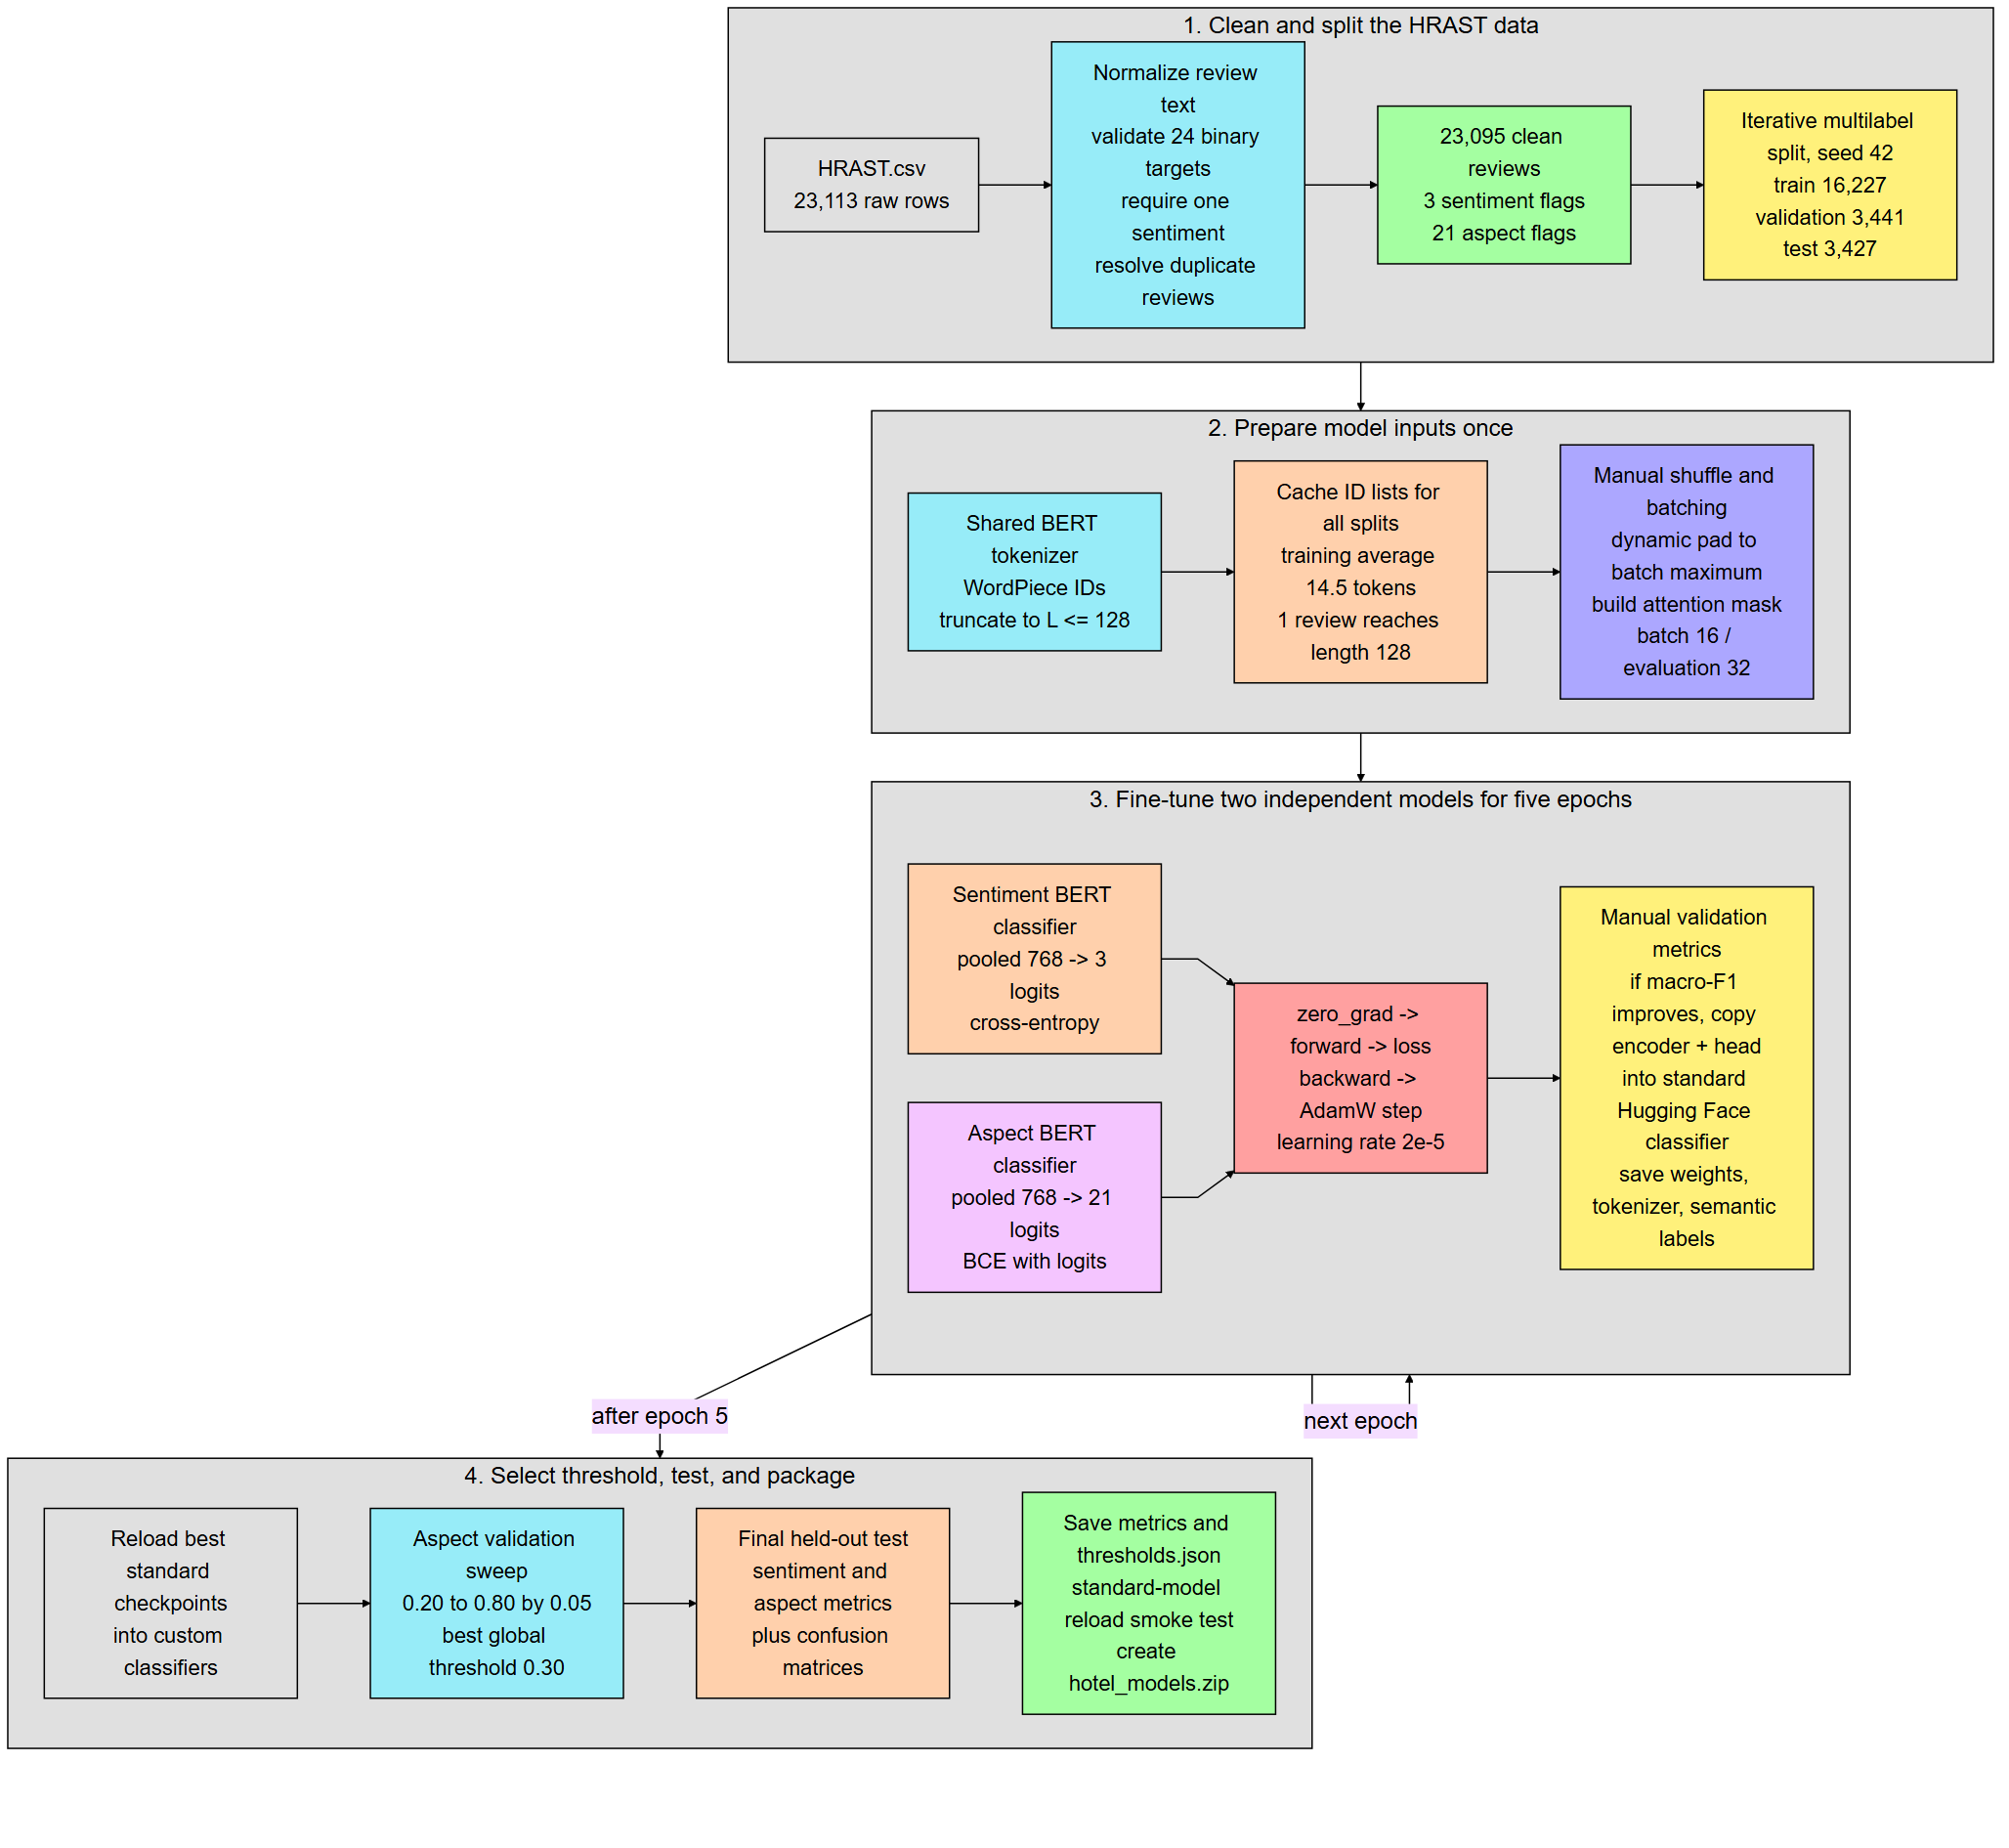
\includegraphics[width=1.18\textwidth,height=0.88\textheight,keepaspectratio]{training_flow.png}}
\caption[Complete model-training flow.]{Complete training, checkpoint-selection, threshold-tuning, and test flow.  Mermaid source: \code{training\_flow.mmd}.}
\label{fig:training-flow}
\end{figure}

\section{Evaluation definitions}

For a class or aspect, let TP, FP, FN, and TN denote the usual confusion counts.  Then
\begin{align}
  \operatorname{Precision}&=\frac{\mathrm{TP}}{\mathrm{TP}+\mathrm{FP}},&
  \operatorname{Recall}&=\frac{\mathrm{TP}}{\mathrm{TP}+\mathrm{FN}},\\
  F_1&=\frac{2\,\mathrm{TP}}{2\,\mathrm{TP}+\mathrm{FP}+\mathrm{FN}},&
  \operatorname{Accuracy}&=\frac{\text{correct sentiment predictions}}{N}.
\end{align}
Macro-F1 gives every label equal importance:
\begin{equation}
  F_{1,\mathrm{macro}}=\frac{1}{C}\sum_{c=1}^{C}F_{1,c}.
\end{equation}
Micro-F1 first pools counts over labels:
\begin{equation}
  F_{1,\mathrm{micro}}=
  \frac{2\sum_c\mathrm{TP}_c}
  {2\sum_c\mathrm{TP}_c+\sum_c\mathrm{FP}_c+\sum_c\mathrm{FN}_c}.
\end{equation}
Macro-F1 exposes weak rare labels; micro-F1 is more strongly influenced by common labels.

\chapter{Results}

\section{Provenance of reported numbers}

The updated notebook contains executed outputs for cleaning, splitting, all five epochs, validation threshold selection, held-out testing, inference examples, and the final reload check.  The empirical figures in this chapter are extracted directly from those cell outputs; the same final values are written to \sourcepath{artifacts/sentiment/metrics.json} and \sourcepath{artifacts/aspects/metrics.json} by the notebook.  This aligns the 3,427 test examples with the reported sentiment supports and aspect confusion counts.

\section{Training dynamics}

\begin{table}[H]
\centering
\caption{Epoch history printed by the updated notebook.  Aspect scores use threshold 0.50 during checkpoint selection.}
\label{tab:epoch-history}
\small
\resizebox{\textwidth}{!}{%
\begin{tabular}{crrrr@{\qquad}rrrr}
\toprule
& \multicolumn{4}{c}{Sentiment} & \multicolumn{4}{c}{Aspects} \\
\cmidrule(lr){2-5}\cmidrule(lr){6-9}
Epoch & Train loss & Val. loss & Val. acc. & Val. macro-F1 & Train loss & Val. loss & Val. macro-F1 & Val. micro-F1 \\
\midrule
1 & 0.2245 & 0.1784 & 0.9404 & 0.6725 & 0.1639 & 0.0862 & 0.6315 & 0.8420 \\
2 & 0.1324 & 0.2094 & 0.9390 & 0.7194 & 0.0659 & 0.0611 & 0.8402 & 0.8786 \\
3 & 0.0884 & 0.2222 & 0.9384 & 0.7145 & 0.0434 & 0.0519 & 0.8619 & 0.8892 \\
4 & 0.0561 & 0.2718 & 0.9425 & 0.7032 & 0.0308 & 0.0513 & 0.8837 & 0.8909 \\
5 & 0.0357 & 0.3156 & 0.9396 & 0.7394 & 0.0223 & 0.0529 & 0.8800 & 0.8896 \\
\bottomrule
\end{tabular}
}
\end{table}

\begin{figure}[H]
\centering
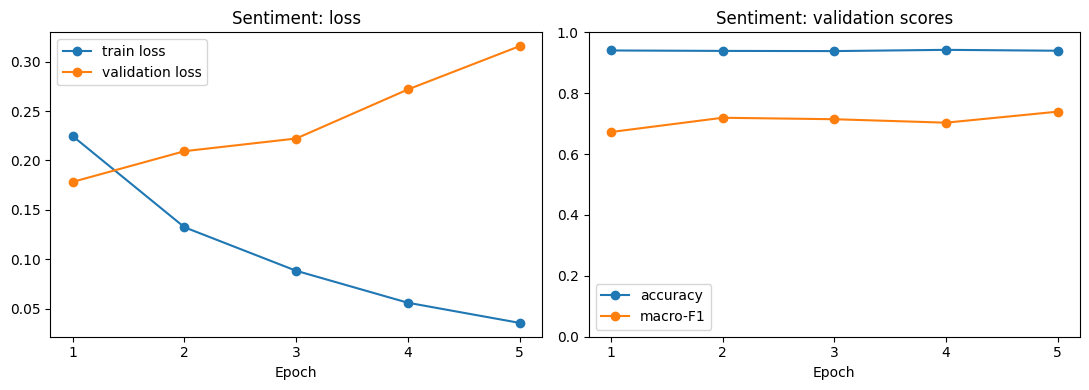
\includegraphics[width=\textwidth]{notebook_sentiment_training_curves.png}
\caption{Empirical sentiment training and validation trajectories.  Training loss falls continuously while validation loss rises after epoch 1; the epoch-5 checkpoint is retained because it gives the highest validation macro-F1.}
\label{fig:sentiment-training-curves}
\end{figure}

\begin{figure}[H]
\centering
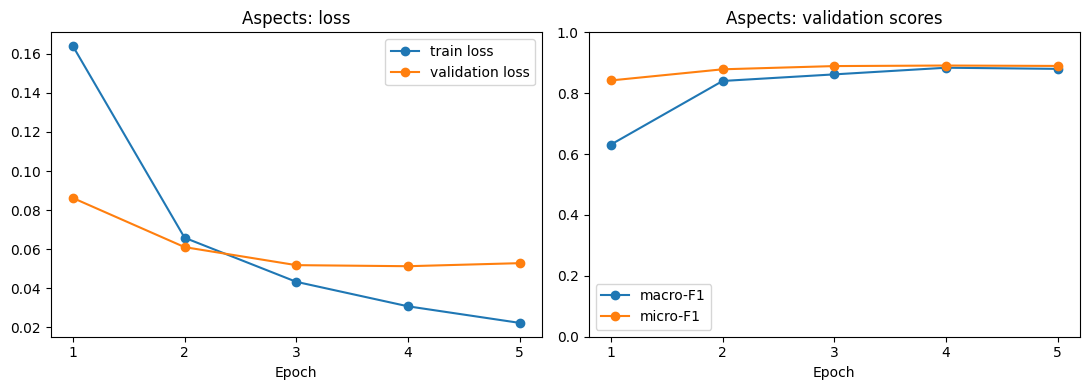
\includegraphics[width=\textwidth]{notebook_aspect_training_curves.png}
\caption{Empirical aspect training and validation trajectories.  Validation macro-F1 peaks at 0.8837 in epoch 4, so that checkpoint is used for threshold selection and testing.}
\label{fig:aspect-training-curves}
\end{figure}

The divergence between decreasing training loss and increasing sentiment validation loss is evidence of overfitting, even though the selection metric recovers its highest value in epoch 5.  For aspects, validation loss is lowest around epochs 3--4 and then increases slightly, consistent with selecting epoch 4.

\section{Aspect threshold selection}

\begin{figure}[H]
\centering
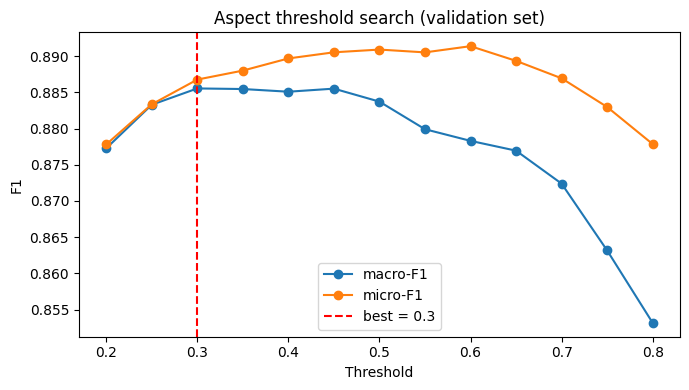
\includegraphics[width=0.82\textwidth]{notebook_aspect_threshold_search.png}
\caption{Validation threshold sweep from 0.20 to 0.80 in steps of 0.05.  Macro-F1 reaches its maximum of 0.8856 at \(\tau=0.30\); micro-F1 peaks at a different threshold, but macro-F1 is the declared selection objective.}
\label{fig:threshold-search}
\end{figure}

At the default threshold 0.50, the held-out aspect test yields macro-F1 0.8820 and micro-F1 0.8976.  After selecting 0.30 exclusively on validation data, the final test macro-F1 becomes 0.8825 and micro-F1 becomes 0.8941.  The change trades a small amount of micro-F1 for the selected macro-F1 objective.

\section{Overall test metrics}

\begin{table}[H]
\centering
\caption{Final held-out test metrics printed and saved by the updated notebook.}
\label{tab:overall-results}
\begin{tabular}{lccc}
\toprule
Task & Accuracy & Macro-F1 & Micro-F1 \\
\midrule
Sentiment & 0.9387 & 0.7258 & --- \\
Aspects (\(\tau=0.30\)) & --- & 0.8825 & 0.8941 \\
\bottomrule
\end{tabular}
\end{table}

\section{Sentiment results}

\begin{table}[H]
\centering
\caption{Sentiment class results on the 3,427-review test set.}
\label{tab:sentiment-results}
\begin{tabular}{lrrrr}
\toprule
Class & Precision & Recall & F1 & Support \\
\midrule
Negative & 0.9406 & 0.9746 & 0.9573 & 1,575 \\
Neutral  & 0.2935 & 0.2288 & 0.2571 & 118 \\
Positive & 0.9718 & 0.9544 & 0.9630 & 1,734 \\
\bottomrule
\end{tabular}
\end{table}

\begin{table}[H]
\centering
\caption{Sentiment confusion matrix (rows are true labels; columns are predictions).}
\label{tab:sentiment-confusion}
\begin{tabular}{lrrr}
\toprule
 & Pred. negative & Pred. neutral & Pred. positive \\
\midrule
True negative & \cellcolor{PaletteGreen}1535 & \cellcolor{PaletteYellow}22 & \cellcolor{PaletteYellow}18 \\
True neutral  & \cellcolor{PaletteRed}61 & \cellcolor{PaletteOrange}27 & \cellcolor{PaletteRed}30 \\
True positive & \cellcolor{PaletteYellow}36 & \cellcolor{PaletteRed}43 & \cellcolor{PaletteGreen}1655 \\
\bottomrule
\end{tabular}
\end{table}

The dominant positive and negative classes both exceed 0.95 F1, but neutral F1 is only 0.2571.  Thus the high overall accuracy hides a substantial minority-class failure, while macro-F1 makes the issue visible.  The confusion matrix shows that most missed neutral reviews are absorbed by negative or positive predictions.

\section{Aspect results}

\begin{longtable}{p{4.3cm}rrrr}
\caption{Per-aspect test results at the selected global threshold 0.30.}\label{tab:aspect-results}\\
\toprule
Aspect & Precision & Recall & F1 & Support \\
\midrule
\endfirsthead
\multicolumn{5}{c}{\tablename\ \thetable{} -- continued}\\
\toprule
Aspect & Precision & Recall & F1 & Support \\
\midrule
\endhead
\midrule
\multicolumn{5}{r}{Continued on next page}\\
\endfoot
\bottomrule
\endlastfoot
Clean & 0.9452 & 0.9431 & 0.9441 & 439 \\
Comfort & 0.8223 & 0.9036 & 0.8610 & 384 \\
Facilities/Amenities & 0.8688 & 0.7995 & 0.8327 & 439 \\
Location & 0.9377 & 0.9549 & 0.9462 & 709 \\
Restaurant (dinner) & 0.4810 & 0.8444 & 0.6129 & 45 \\
Staff & 0.9610 & 0.9509 & 0.9559 & 570 \\
View (Balcony) & 0.8231 & 0.9145 & 0.8664 & 117 \\
Breakfast & 0.9541 & 0.9816 & 0.9677 & 381 \\
Room & 0.7684 & 0.9055 & 0.8313 & 751 \\
Pool & 0.9595 & 1.0000 & 0.9793 & 71 \\
Beach & 0.8800 & 0.7857 & 0.8302 & 28 \\
Bathroom/Shower (toilet) & 0.9178 & 0.9858 & 0.9505 & 351 \\
Bar & 0.8542 & 0.8542 & 0.8542 & 48 \\
Bed & 0.9587 & 0.9414 & 0.9500 & 222 \\
Parking & 0.9634 & 0.9753 & 0.9693 & 81 \\
Noise & 0.9312 & 0.9544 & 0.9426 & 241 \\
Reception-checkin & 0.7207 & 0.9021 & 0.8012 & 143 \\
Lift & 0.9524 & 0.9091 & 0.9302 & 44 \\
Value for money & 0.7468 & 0.8647 & 0.8014 & 133 \\
Wi-Fi & 0.9091 & 1.0000 & 0.9524 & 40 \\
Generic & 0.7750 & 0.7331 & 0.7535 & 296 \\
\end{longtable}

\subsection{Per-aspect confusion matrices}

Each aspect is an independent binary decision, so it has a \(2\times2\) confusion matrix rather than one shared 21-class matrix.  The following counts use the updated notebook's \(N=3{,}427\) test reviews.  Rows are ground truth and columns are predictions; green cells are correct decisions, red cells are false positives, and yellow cells are false negatives.

\begin{figure}[p]
\centering
\aspectcm{Clean}{2964}{24}{25}{414}\hfill
\aspectcm{Comfort}{2968}{75}{37}{347}\hfill
\aspectcm{Facilities/Amenities}{2935}{53}{88}{351}
\par\vspace{0.5cm}
\aspectcm{Location}{2673}{45}{32}{677}\hfill
\aspectcm{Restaurant (dinner)}{3341}{41}{7}{38}\hfill
\aspectcm{Staff}{2835}{22}{28}{542}
\par\vspace{0.5cm}
\aspectcm{View (Balcony)}{3287}{23}{10}{107}\hfill
\aspectcm{Breakfast}{3028}{18}{7}{374}\hfill
\aspectcm{Room}{2471}{205}{71}{680}
\par\vspace{0.5cm}
\aspectcm{Pool}{3353}{3}{0}{71}\hfill
\aspectcm{Beach}{3396}{3}{6}{22}\hfill
\aspectcm{Bathroom/Shower}{3045}{31}{5}{346}
\caption{Aspect confusion matrices, part 1 of 2.}
\label{fig:aspect-confusion-1}
\end{figure}

\begin{figure}[p]
\centering
\aspectcm{Bar}{3372}{7}{7}{41}\hfill
\aspectcm{Bed}{3196}{9}{13}{209}\hfill
\aspectcm{Parking}{3343}{3}{2}{79}
\par\vspace{0.6cm}
\aspectcm{Noise}{3169}{17}{11}{230}\hfill
\aspectcm{Reception-checkin}{3234}{50}{14}{129}\hfill
\aspectcm{Lift}{3381}{2}{4}{40}
\par\vspace{0.6cm}
\aspectcm{Value for money}{3255}{39}{18}{115}\hfill
\aspectcm{Wi-Fi}{3383}{4}{0}{40}\hfill
\aspectcm{Generic}{3068}{63}{79}{217}
\caption{Aspect confusion matrices, part 2 of 2.}
\label{fig:aspect-confusion-2}
\end{figure}

\begin{figure}[H]
\centering
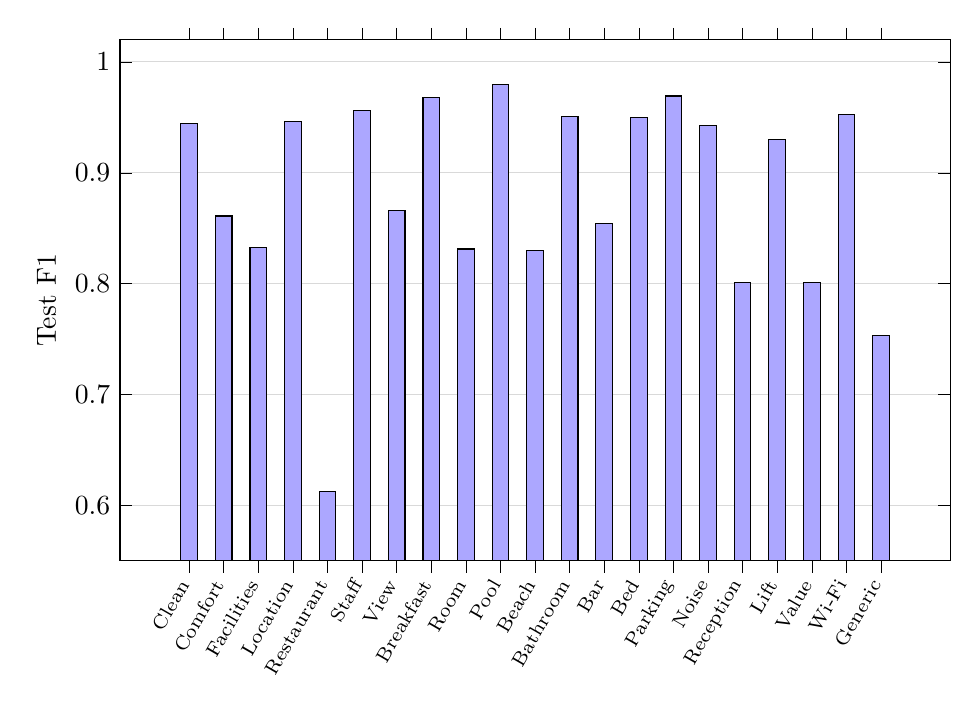
\begin{tikzpicture}
\begin{axis}[
  width=\textwidth,
  height=8.2cm,
  ybar,
  bar width=6pt,
  ymin=0.55,ymax=1.02,
  ylabel={Test F1},
  symbolic x coords={Clean,Comfort,Facilities,Location,Restaurant,Staff,View,Breakfast,Room,Pool,Beach,Bathroom,Bar,Bed,Parking,Noise,Reception,Lift,Value,Wi-Fi,Generic},
  xtick=data,
  x tick label style={rotate=60,anchor=east,font=\scriptsize},
  ymajorgrids=true,
  grid style={black!15},
  axis line style={black},
  tick style={black},
  every axis plot/.append style={draw=black},
]
\addplot[fill=PalettePurple] coordinates {
 (Clean,0.9441) (Comfort,0.8610) (Facilities,0.8327) (Location,0.9462)
 (Restaurant,0.6129) (Staff,0.9559) (View,0.8664) (Breakfast,0.9677)
 (Room,0.8313) (Pool,0.9793) (Beach,0.8302) (Bathroom,0.9505)
 (Bar,0.8542) (Bed,0.9500) (Parking,0.9693) (Noise,0.9426)
 (Reception,0.8012) (Lift,0.9302) (Value,0.8014) (Wi-Fi,0.9524)
 (Generic,0.7535)};
\end{axis}
\end{tikzpicture}
\caption{Per-aspect test F1 from the updated notebook.  Restaurant (dinner) is the weakest aspect because precision is only 0.4810; this is consistent with its low support.}
\label{fig:aspect-f1}
\end{figure}

The aspect model is more balanced than the sentiment model across its labels, but the rare Restaurant (dinner) category has a clear precision problem.  Room, Reception-checkin, Value for money, Generic, and Facilities/Amenities are the next most important improvement targets.

\chapter{Inference Web Demo}

\section{Runtime behavior}

The Streamlit application searches for a parent directory containing both \sourcepath{sentiment/config.json} and \sourcepath{aspects/config.json}.  Its search order is the \code{HOTEL\_MODELS\_DIR} environment variable, \sourcepath{artifacts}, and \sourcepath{hotel_models/artifacts}.  It then:
\begin{enumerate}[leftmargin=*]
  \item selects CUDA when available, otherwise CPU;
  \item loads both tokenizers and models once through \code{@st.cache\_resource};
  \item loads \code{global\_threshold} from \sourcepath{aspects/thresholds.json}, with a 0.50 fallback;
  \item accepts an example or user-entered review and optionally overrides the aspect threshold with a sidebar slider;
  \item tokenizes to at most 128 tokens and executes both models under \code{torch.no\_grad()};
  \item applies softmax and argmax for sentiment, and independent sigmoid thresholding for aspects;
  \item displays a sentiment confidence chart, detected-aspect progress bars, and an expandable chart of all 21 aspect probabilities.
\end{enumerate}

\begin{figure}[H]
\centering
\makebox[\textwidth][c]{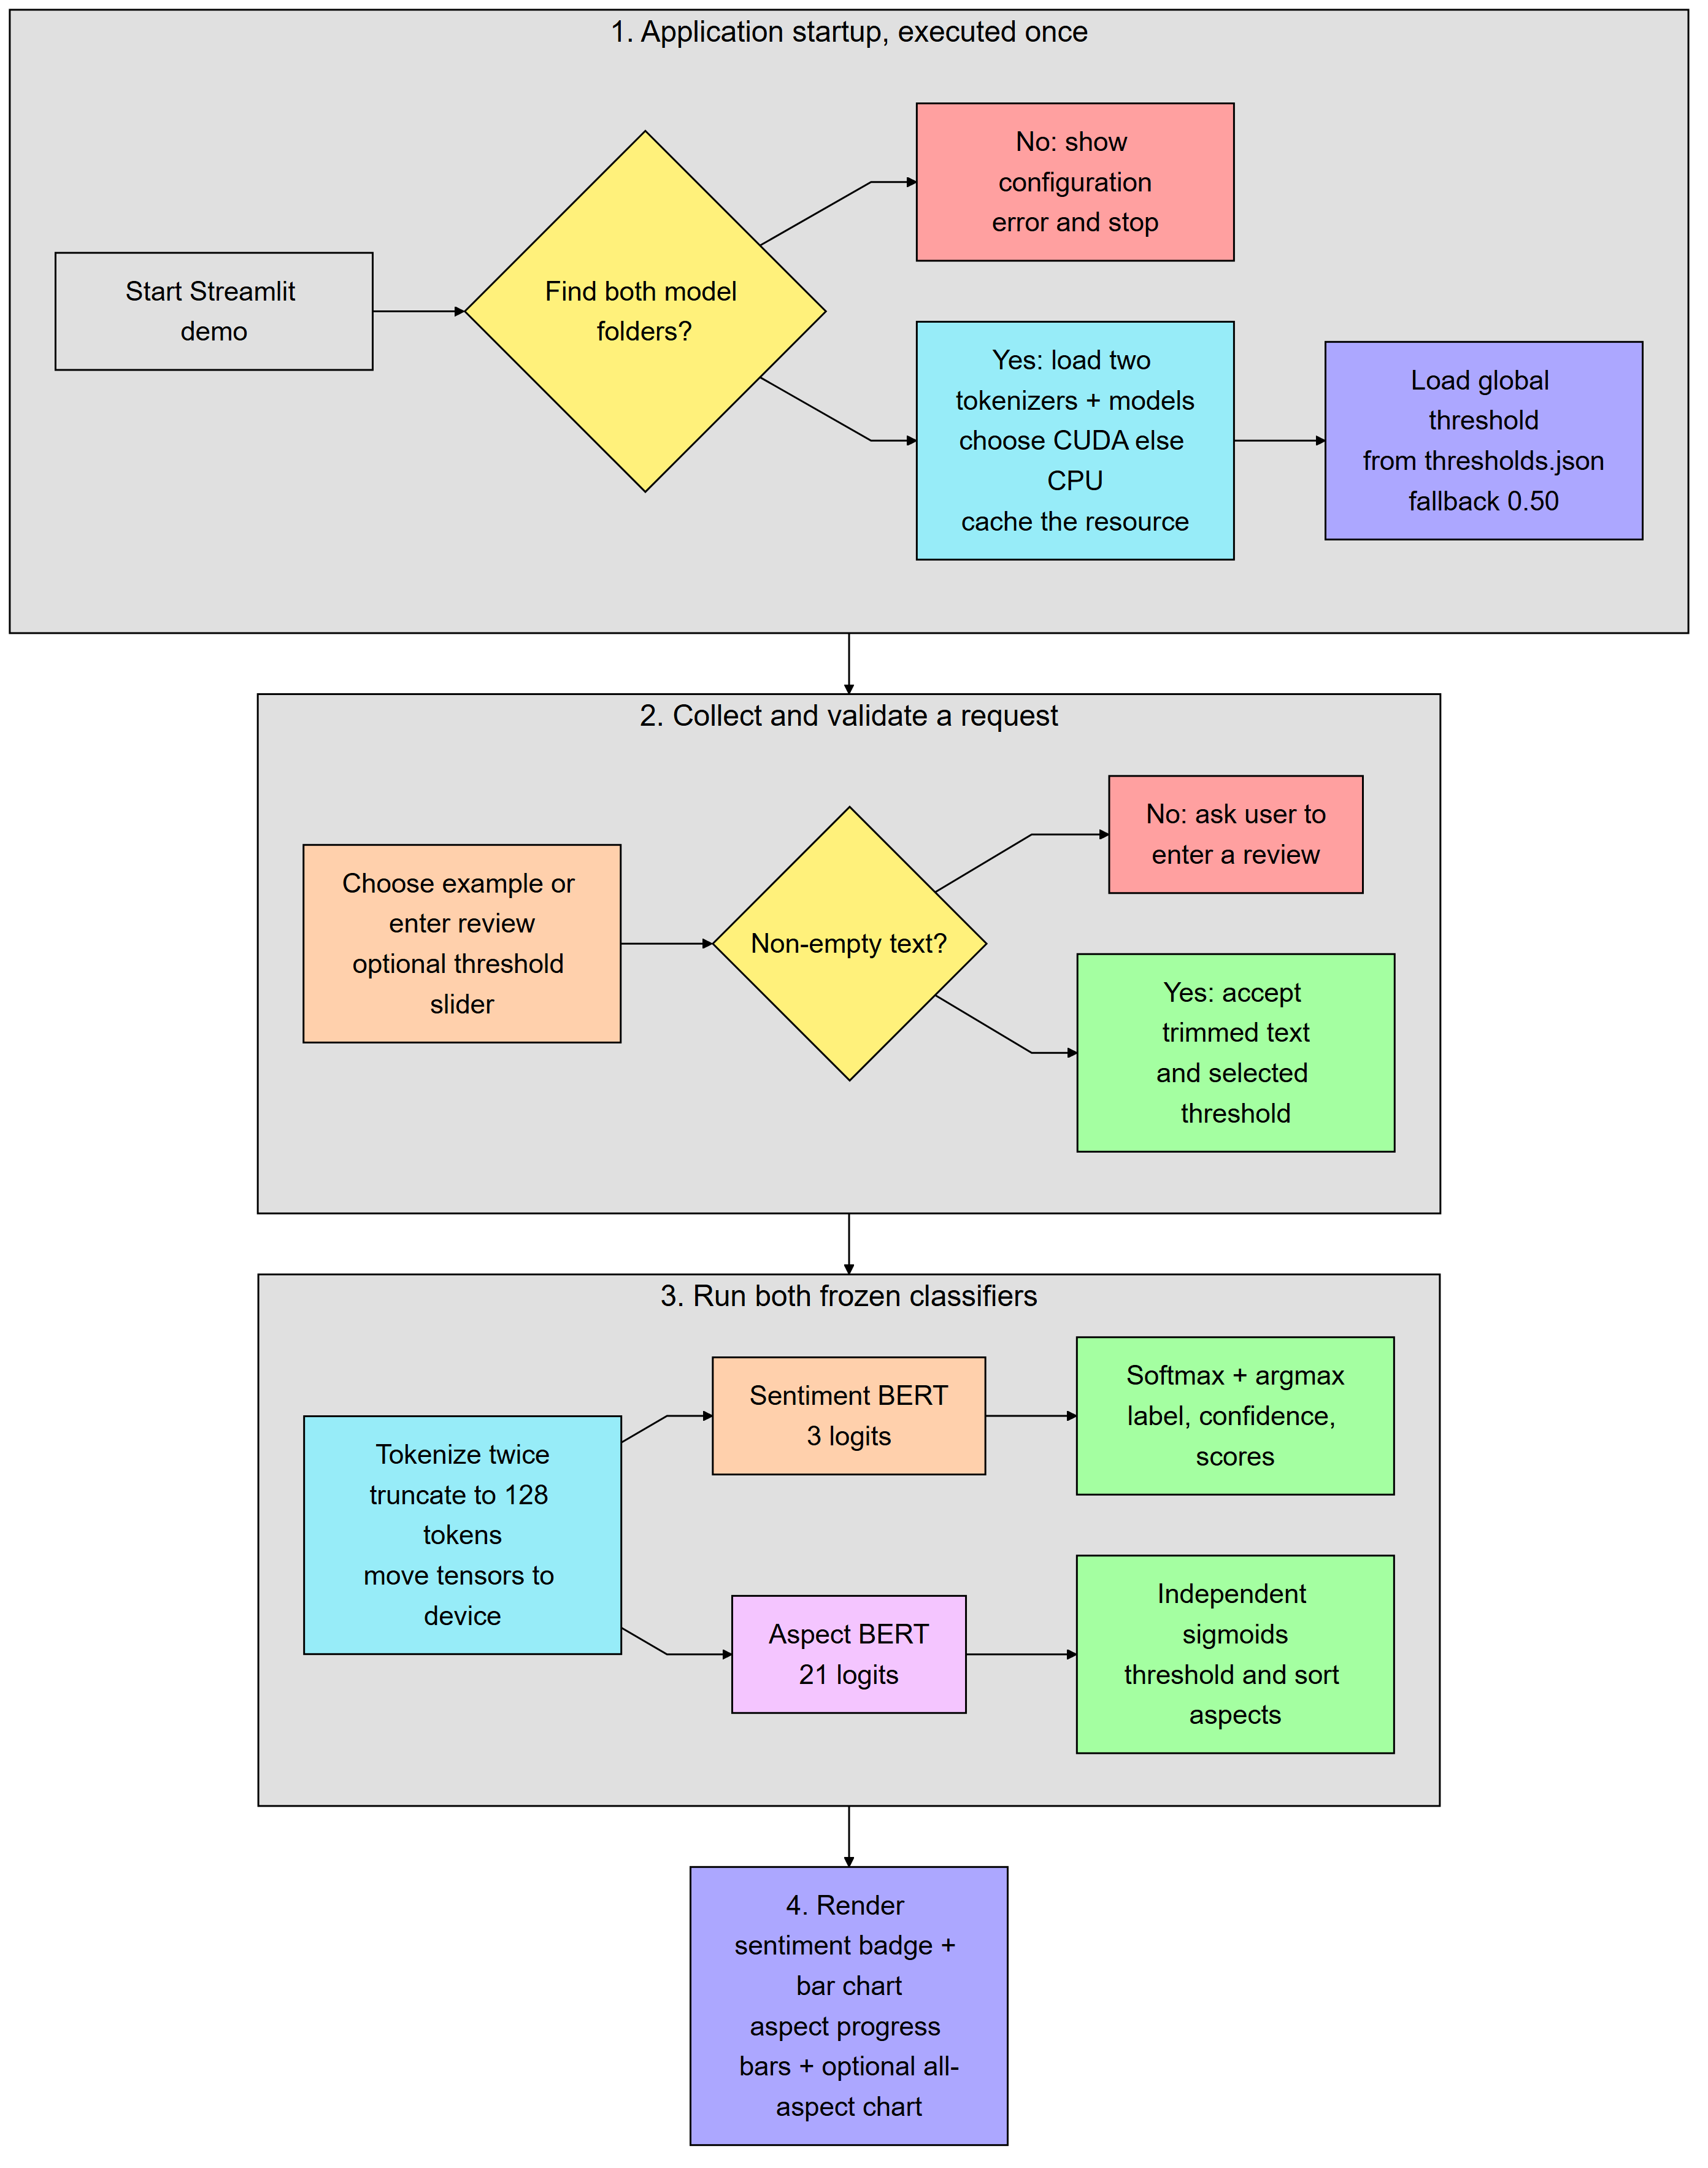
\includegraphics[width=1.18\textwidth,height=0.82\textheight,keepaspectratio]{inference_flow.png}}
\caption[Streamlit inference flow.]{Streamlit inference and presentation flow.  Mermaid source: \code{inference\_flow.mmd}.}
\label{fig:inference-flow}
\end{figure}

For a single review, the sentiment output is a dictionary of three probabilities plus their maximum label.  Aspect probabilities do not sum to one; the app retains every label satisfying \(p_j\geq\tau\) and sorts retained labels by probability.

\section{Demonstration screenshots}

Figures~\ref{fig:web-demo-full}--\ref{fig:web-demo-results} show an actual CUDA-backed run of the Streamlit application using the review ``Overall, we had a wonderful time and would definitely come back.''  At the tuned threshold \(\tau=0.30\), the deployed checkpoints return positive sentiment with rounded confidence 100.0\% and detect the Generic aspect at 98.7\%.

\begin{figure}[p]
\centering
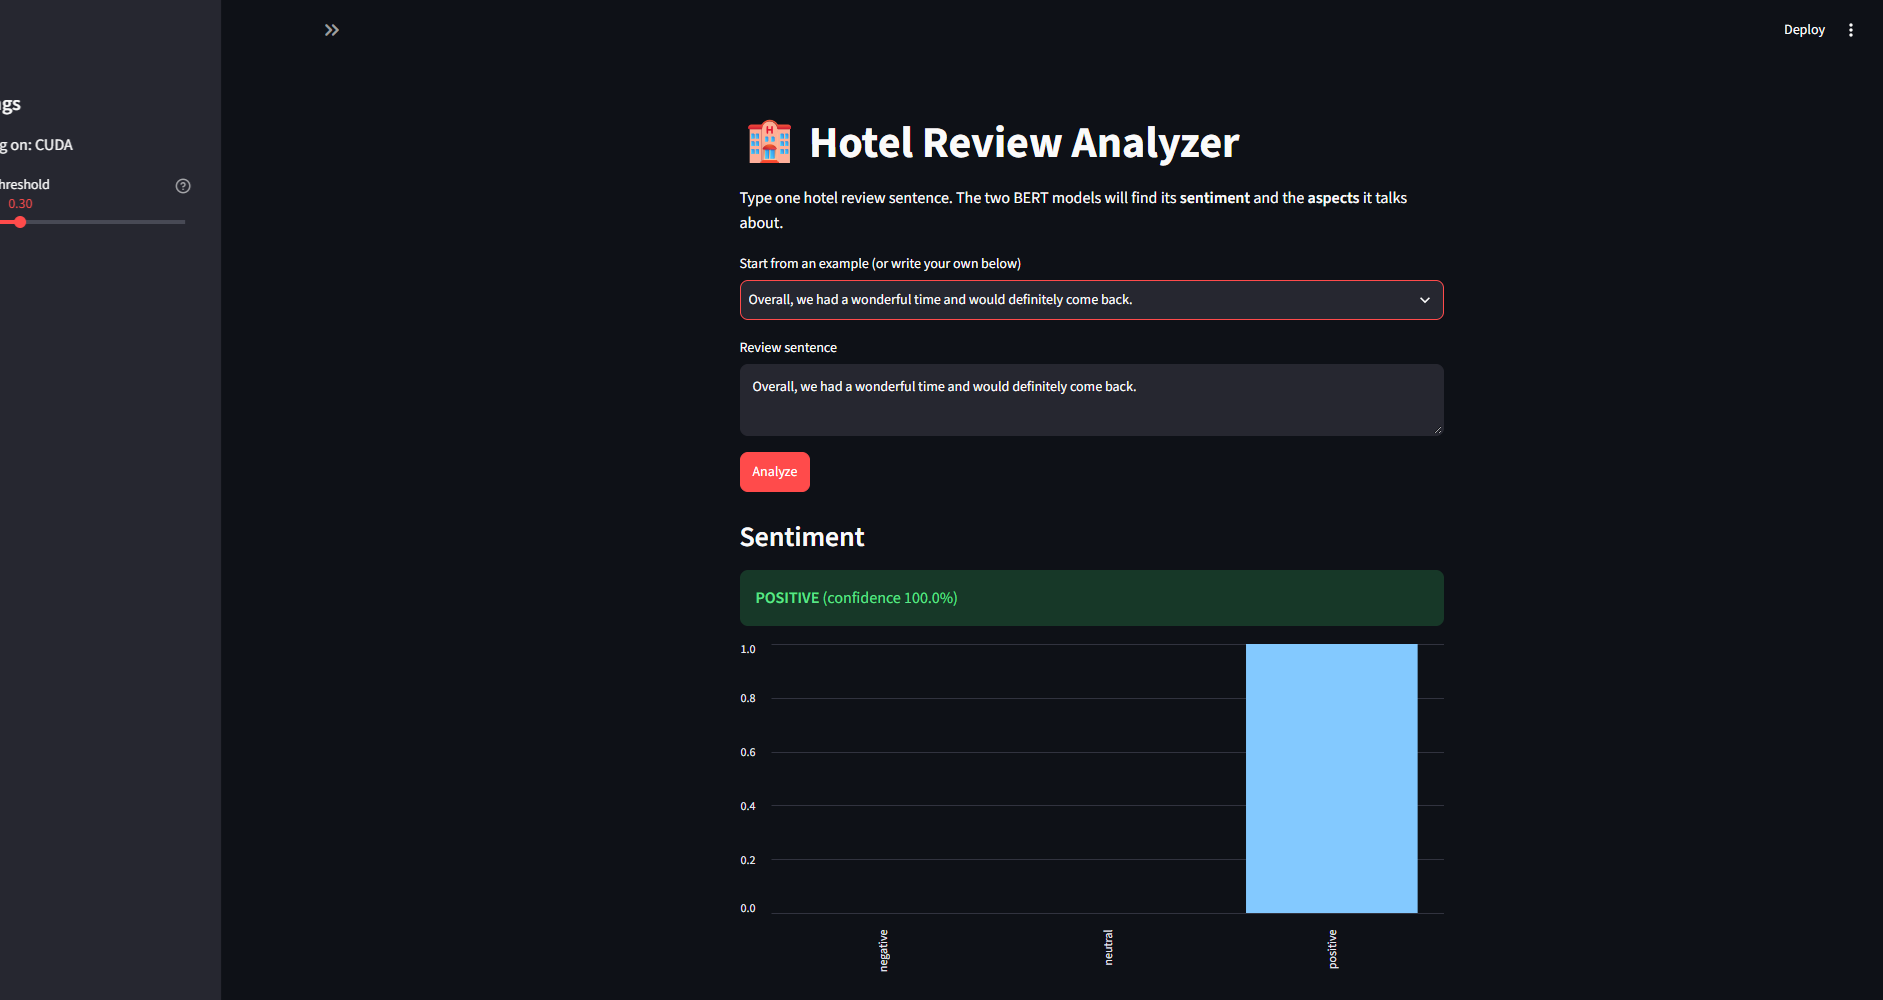
\includegraphics[width=\textwidth]{web_demo_full.png}
\caption{Full Hotel Review Analyzer interface after submitting the example review.}
\label{fig:web-demo-full}
\end{figure}

\begin{figure}[p]
\centering
\begin{subfigure}{0.96\textwidth}
\centering
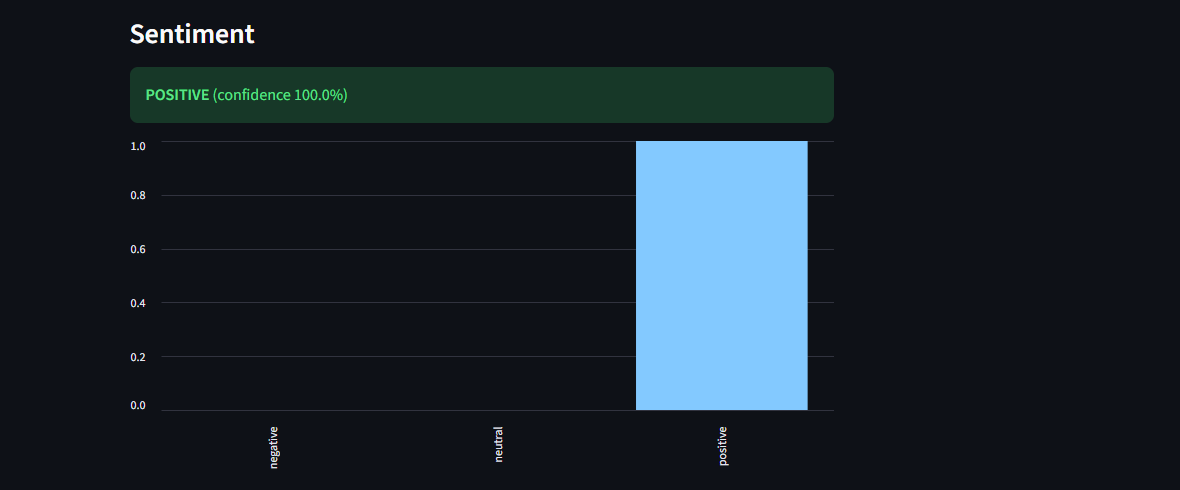
\includegraphics[width=\textwidth]{web_demo_sentiment.png}
\caption{Three-way softmax sentiment output.}
\end{subfigure}

\vspace{0.55cm}
\begin{subfigure}{0.96\textwidth}
\centering
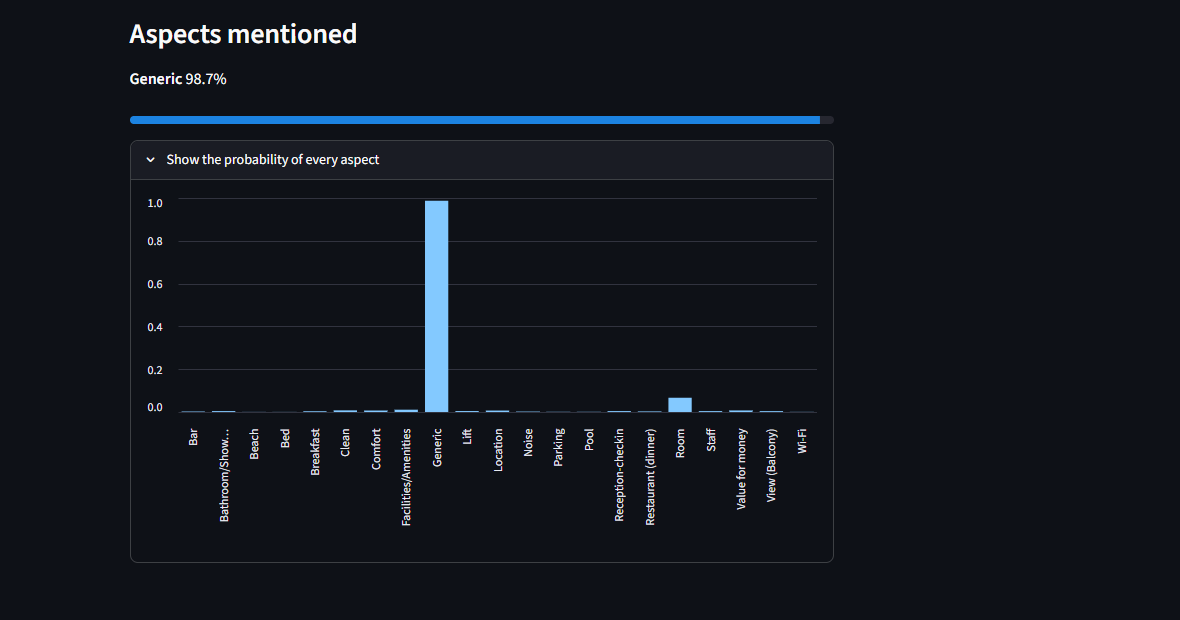
\includegraphics[width=\textwidth]{web_demo_aspects.png}
\caption{Detected aspect and all 21 sigmoid probabilities.}
\end{subfigure}
\caption{Detailed prediction panels produced by the inference web demo.}
\label{fig:web-demo-results}
\end{figure}

\clearpage

\section{Training-to-inference contract verification}

\begin{table}[H]
\centering
\caption{Verified interface between the updated notebook and the web applications.}
\label{tab:compatibility}
\small
\begin{tabularx}{\textwidth}{p{2.8cm}>{\raggedright\arraybackslash}X>{\raggedright\arraybackslash}X}
\toprule
Contract item & Notebook behavior & Verification outcome \\
\midrule
Model format & The export helper copies the custom encoder and classifier weights into a standard Hugging Face sequence classifier and calls \code{save\_pretrained}. & Both Streamlit and Flask can load the resulting folders with the standard Transformers API. \\
Label names & The export includes semantic \code{id2label}, \code{label2id}, and task-specific \code{problem\_type}. & Reloaded sentiment configuration reports \{0: negative, 1: neutral, 2: positive\}; aspect coordinates retain their 21 names. \\
Threshold file & The aspect folder contains plural \code{thresholds.json} with \code{global\_threshold} and \code{per\_label\_thresholds}. & Streamlit reads the global value; the shared Flask predictor can use the per-label mapping. \\
Selection protocol & The best aspect checkpoint is chosen at validation threshold 0.50, then \(\tau^*=0.30\) is selected on validation and used for a separate final test. & Test metrics correspond to the tuned deployment decision rule rather than the pre-tuning default. \\
Reload consistency & The notebook loads the saved tokenizer and standard classifiers exactly as the web path does and compares logits. & Maximum sentiment-logit difference is \(1.1921\times10^{-6}\); reloaded inference detects Staff and Breakfast for the smoke-test review. \\
Deliverables & Each folder contains config, tokenizer files, metrics, and approximately 438 MB of weights; aspects also contain thresholds. & The two folders are packed into \code{hotel\_models.zip} for deployment. \\
\bottomrule
\end{tabularx}
\end{table}

The updated notebook therefore closes the earlier naming and metadata gaps.  Its four printed example predictions also exercise mixed sentiment and multiple aspects, including Staff plus Breakfast and Wi-Fi plus Noise.

\chapter{Limitations and Recommended Improvements}

\begin{enumerate}[leftmargin=*]
  \item \textbf{Neutral-class imbalance.}  The neutral class has very low support and F1.  Compare class-weighted cross-entropy, focal loss, careful neutral oversampling, or a two-stage sentiment design.  Any resampling must occur only inside the training split.
  \item \textbf{Global aspect threshold.}  A single threshold is simple but suboptimal when label prevalence and calibration differ.  Select \(\tau_j\) per aspect on validation data, subject to a minimum-support rule to reduce overfitting rare labels.
  \item \textbf{Run-manifest durability.}  The executed notebook preserves plots and writes final metrics, but epoch histories exist only in cell output and memory.  Export histories to JSON/CSV together with the dataset SHA-256, split indices, package versions, code revision, and checkpoint hashes.
  \item \textbf{Partial reproducibility.}  Seeding Python, NumPy, and PyTorch helps, but GPU kernels may remain nondeterministic.  Enable deterministic algorithms when bitwise reruns are required and record the Tesla T4 software environment.
  \item \textbf{Truncation.}  Only one of 16,227 training reviews reaches the 128-token cap, so observed truncation exposure is extremely small in this split.  Still monitor this statistic when the data source changes; longer production reviews may require 256 tokens, head-tail truncation, or sentence-level aggregation.
  \item \textbf{Calibration and abstention.}  Confidence is displayed as if calibrated.  Reliability diagrams, expected calibration error, temperature scaling for sentiment, and per-label calibration for aspects should be evaluated before high-stakes use.
  \item \textbf{Deployment efficiency.}  Two independent BERT-base models approximately double memory and latency.  A shared encoder with two task heads could reduce cost, but it changes the learning problem and must be benchmarked against the current independent-model baseline.
  \item \textbf{Input validation.}  The Flask implementation enforces a 2,000-character limit, while the Streamlit demo accepts arbitrary text before token truncation.  Align validation and user-facing error behavior across interfaces.
\end{enumerate}

\chapter{Conclusion}

The project correctly separates single-label sentiment from multilabel aspect detection and applies the appropriate probability transforms and losses to each.  Its preprocessing removes malformed and contradictory records before a multilabel-stratified 70/15/15 split.  BERT-base supplies a 12-layer, 768-dimensional encoder, while task-specific linear heads produce either three mutually exclusive logits or 21 independent logits.  AdamW fine-tunes the full networks, validation macro-F1 selects checkpoints, and validation threshold search controls aspect decisions.

The aspect model reports strong and reasonably balanced performance, whereas neutral sentiment remains the dominant weakness.  The updated notebook now persists final metrics, saves semantic label mappings, writes the threshold filename and structure expected by inference, evaluates the selected threshold on the held-out test set, reloads the deployed format, and produces a downloadable archive.  Persisting the epoch histories and a cryptographic run manifest would complete the remaining reproducibility work.

\appendix
\chapter{Diagram Sources and Palette}

Every architecture or process diagram in this report is stored as editable Mermaid source in the same directory as this file:
\begin{itemize}[leftmargin=*]
  \item \sourcepath{bert_architecture.mmd}
  \item \sourcepath{training_flow.mmd}
  \item \sourcepath{inference_flow.mmd}
\end{itemize}
The rendered PNG files are generated from these sources for LaTeX inclusion.  Node fills are restricted to the supplied palette, text is black, and connector strokes and arrowheads are black.

\begin{table}[H]
\centering
\caption{Diagram color palette.}
\begin{tabular}{ll@{\qquad}ll}
\toprule
Color & Hex & Color & Hex \\
\midrule
\cellcolor{PaletteGray}Gray & \#E0E0E0 & \cellcolor{PaletteCyan}Cyan & \#97ECF8 \\
\cellcolor{PaletteOrange}Orange & \#FFD0AC & \cellcolor{PaletteRed}Red & \#FFA0A0 \\
\cellcolor{PaletteYellow}Yellow & \#FFF17B & \cellcolor{PalettePurple}Purple & \#ACA7FF \\
\cellcolor{PaletteGreen}Green & \#A4FFA1 & \cellcolor{PalettePink}Pink & \#F4C5FF \\
\bottomrule
\end{tabular}
\end{table}

\begin{thebibliography}{9}

\bibitem{devlin2019}
J. Devlin, M.-W. Chang, K. Lee, and K. Toutanova,
``BERT: Pre-training of Deep Bidirectional Transformers for Language Understanding,''
\emph{Proceedings of NAACL-HLT}, 2019.

\bibitem{loshchilov2019}
I. Loshchilov and F. Hutter,
``Decoupled Weight Decay Regularization,''
\emph{International Conference on Learning Representations}, 2019.

\bibitem{sechidis2011}
K. Sechidis, G. Tsoumakas, and I. Vlahavas,
``On the Stratification of Multi-label Data,''
\emph{European Conference on Machine Learning and Principles and Practice of Knowledge Discovery in Databases}, 2011.

\end{thebibliography}

\end{document}
